\documentclass[twoside]{article}

% Some basic packages
\usepackage[utf8]{inputenc}
\usepackage[T1]{fontenc}
\usepackage{textcomp}
\usepackage{url}
\usepackage{graphicx}
\usepackage{float}
\usepackage{booktabs}
\usepackage{enumitem}

% Don't indent paragraphs.
\usepackage{parskip}

% Hide page number when page is empty
\usepackage{emptypage}
\usepackage{subcaption}
\usepackage{multicol}
\usepackage{xcolor}

% Math stuff
\usepackage{amsmath, amsfonts, mathtools, amsthm, amssymb}
% Non-ams math stuff
\usepackage{derivative, physics}
% Fancy script capitals
\usepackage{mathrsfs}
\usepackage{cancel}

% Bold math
\usepackage{bm}

% Cool command shortcuts
\newcommand\N{\ensuremath{\mathbb{N}}}
\newcommand\R{\ensuremath{\mathbb{R}}}
\newcommand\Z{\ensuremath{\mathbb{Z}}}
\renewcommand\O{\ensuremath{\emptyset}}
\newcommand\Q{\ensuremath{\mathbb{Q}}}
\newcommand\C{\ensuremath{\mathbb{C}}}

% Operators
\DeclareMathOperator*{\argmax}{arg\,max}
\DeclareMathOperator*{\argmin}{arg\,min}

% Easily typeset systems of equations (French package)
\usepackage{systeme}

%Make implies and impliedby shorter
\let\implies\Rightarrow
\let\impliedby\Leftarrow
\let\iff\Leftrightarrow
\let\epsilon\varepsilon
\let\phi\varphi

% Add \contra symbol to denote contradiction
\usepackage{stmaryrd} % for \lightning
\newcommand\contra{\scalebox{1.5}{$\lightning$}}

% horizontal rule
\newcommand\hr{
    \noindent\rule[0.5ex]{\linewidth}{0.5pt}
}

% For box around Definition, Theorem, \ldots
\usepackage{mdframed}
\mdfsetup{skipabove=1em,skipbelow=0em}
\theoremstyle{definition}
\newmdtheoremenv[nobreak=true]{definition}{Definition}
\newmdtheoremenv[nobreak=true]{lemma}{Lemma}
\newmdtheoremenv[nobreak=true]{proposition}{Proposition}
\newmdtheoremenv[nobreak=true]{theorem}{Theorem}
\newmdtheoremenv[nobreak=true]{corollary}{Corollary}
\newmdtheoremenv{conjecture}{Conjecture}
\newtheorem*{remark}{Remark}
\newtheorem*{problem}{Problem}
\newtheorem*{eg}{Example}
\newtheorem*{question}{Question}
\newtheorem*{intuition}{Intuition}
\newtheorem*{claim}{Claim}

% End example environments with a small diamond (just like proof
% environments end with a small square)
\usepackage{etoolbox}
\AtEndEnvironment{eg}{\null\hfill$\diamond$}%

% Fix some spacing
% http://tex.stackexchange.com/questions/22119/how-can-i-change-the-spacing-before-theorems-with-amsthm
\makeatletter
\def\thm@space@setup{%
  \thm@preskip=\parskip \thm@postskip=0pt
}

% Exercise 
% Usage:
% \oefening{5}
% \suboefening{1}
% \suboefening{2}
% \suboefening{3}
% gives
% Oefening 5
%   Oefening 5.1
%   Oefening 5.2
%   Oefening 5.3
\newcommand{\exercise}[1]{%
    \def\@exercise{#1}%
    \subsection*{Exercise #1}
}

\newcommand{\subexercise}[1]{%
    \subsubsection*{Exercise \@exercise.#1}
}

% \lecture starts a new lecture (les in dutch)
%
% Usage:
% \lecture{1}{di 12 feb 2019 16:00}{Inleiding}
%
% This adds a section heading with the number / title of the lecture and a
% margin paragraph with the date.

% I use \dateparts here to hide the year (2019). This way, I can easily parse
% the date of each lecture unambiguously while still having a human-friendly
% short format printed to the pdf.

\usepackage{xifthen}
\def\testdateparts#1{\dateparts#1\relax}
\def\dateparts#1 #2 #3 #4 #5\relax{
    \marginpar{\small\textsf{\mbox{#1 #2 #3 #5}}}
}

\def\@lecture{}%
\newcommand{\lecture}[3]{
    \ifthenelse{\isempty{#3}}{%
        \def\@lecture{Lecture #1}%
    }{%
        \def\@lecture{Lecture #1: #3}%
    }%
    \subsection*{\@lecture}
    \marginpar{\small\textsf{\mbox{#2}}}
}


% For page size and geometry
\usepackage{geometry}

% These are the fancy headers
\usepackage{fancyhdr}
\pagestyle{fancy}

% LE: left even
% RO: right odd
% CE, CO: center even, center odd
% My name for when I print my lecture notes to use for an open book exam.
% \fancyhead[LE,RO]{Gilles Castel}

\fancyhead[RO,LE]{\@lecture} % Right odd,  Left even
\fancyhead[RE,LO]{}          % Right even, Left odd

\fancyfoot[RO,LE]{\thepage}  % Right odd,  Left even
\fancyfoot[RE,LO]{}          % Right even, Left odd
\fancyfoot[C]{\leftmark}     % Center

\makeatother

% Todonotes and inline notes in fancy boxes
\usepackage{todonotes}
\usepackage{tcolorbox}

% Fix some stuff
% %http://tex.stackexchange.com/questions/76273/multiple-pdfs-with-page-group-included-in-a-single-page-warning
\pdfsuppresswarningpagegroup=1


% name
\author{Asier García Ruiz}

\usetikzlibrary{shapes.geometric, arrows}

\title{Deep Learning Problem Set 2}
\begin{document}
\maketitle

\exercise{1}
I collaborated with Ayush Panda on this homework.

\exercise{2}
\subexercise{1}
\begin{proof}
	We are to find the solution $\bm{w}^{*}$ to the following problem
	\begin{equation*}
		\argmin_{\bm{w}} f(\bm{w}^{(t)}) + \langle \bm{w} - \bm{w}^{(t)}, \grad f(\bm{w}^{(t)})
		+ \frac{\lambda}{2} \lVert \bm{w} - \bm{w}^{(t)} \rVert^{2}.
	\end{equation*}
	Since there are no constraints and $f$ is convex, we can simply define the function
	\begin{equation*}
		\mathcal{L}(\bm{w}) = f(\bm{w}^{(t)}) + \langle \bm{w} - \bm{w}^{(t)}, \grad f(\bm{w}^{(t)})
		+ \frac{\lambda}{2} \lVert \bm{w} - \bm{w}^{(t)} \rVert^{2}
	\end{equation*}
	and find the minimum by taking the gradient.

	\begin{claim}
		We claim that
		\begin{equation*}
			\grad \lVert \bm{x} \rVert^{2} = 2\bm{x}.
		\end{equation*}
		\begin{proof}
			From the definiton of the norm
			\begin{equation*}
				f(x) = \lVert \bm{x} \rVert^{2} = \sum_{j = 1}^{n} x_{j}^{2},
			\end{equation*}
			then
			\begin{equation*}
				\pdv{f}{x_{i}} = \pdv{}{x_{i}} \sum_{j = 1}^{n} x_{j}^{2} = 2x_{i}
			\end{equation*}
			and the claim follows.
		\end{proof}
	\end{claim}

	Having proven this claim, we proceed to find $\grad \mathcal{L}(\bm{w})$. We write,
	\begin{align*}
		\grad_{\bm{w}} \mathcal{L}(\bm{W}) & = \grad_{\bm{w}}
		\left[ f(\bm{w}^{(t)}) + \langle \bm{w} - \bm{w}^{(t)}, \grad f(\bm{w}^{(t)})\rangle
		+ \frac{\lambda}{2} \lVert \bm{w} - \bm{w}^{(t)} \rVert^{2} \right],                               \\
		                                   & = 0 + \grad f(\bm{w}^{(t)}) + \lambda(\bm{w} - \bm{w}^{(t)}). \\
	\end{align*}
	Now, setting this equal to zero, we get
	\begin{equation*}
		\bm{w} = \bm{w}^{(t)} - \frac{1}{\lambda}\grad f(\bm{w}^{(t)}).
	\end{equation*}

	This tells us that the gradient descent method is the solution to this $\argmin$ problem. Meaning that
	assuming that $f$ is convex (or at least locally convex) it will always take us towards the $\bm{w}^{*}$
	that minimises this loss function, should we choose to use it.

	Clearly we can see that $\eta = \frac{1}{\lambda}$.
\end{proof}

\subexercise{2}
\begin{proof}
	We will prove the inequality
	\begin{equation*}
		\sum_{t=1}^{T} \langle \bm{w}^{(t)} - \bm{w}^{*}, \bm{v}_{t}\rangle
		\leq \frac{\lVert \bm{w}^{*} \rVert^{2}}{2 \eta}
		+ \frac{\eta}{2}\sum_{t=1}^{T}\lVert \bm{v}_{t} \rVert^{2}.
	\end{equation*}

	We begin by noting that
	\begin{align*}
		\lVert \bm{w}^{(t+1)} - \bm{w}^{(*)} \rVert^{2}
		 & = \lVert \bm{w}^{(t)} - \eta \bm{v}_{t} - \bm{w}^{*} \rVert^{2},                                     \\
		 & = \lVert \bm{w}^{(t)} - \bm{w}^{*} \rVert^{2}
		+ \eta^{2} \lVert \bm{v}_{t} \rVert^{2} - 2 \eta \langle \bm{w}^{(t)} - \bm{w}^{*}, \bm{v}_{t} \rangle. \\
	\end{align*}
	Which, after rearranging gives us
	\begin{equation*}
		\langle \bm{w}^{(t)} - \bm{w}^{*}, \bm{v}_{t} \rangle
		= \frac{\lVert \bm{w}^{(t)} - \bm{w}^{*} \rVert^{2}}{2 \eta}
		+ \frac{\eta \lVert \bm{v}_{t} \rVert^{2}}{2}
		-  \frac{\lVert \bm{w}^{(t + 1)} - \bm{w}^{*} \rVert^{2}}{2 \eta}.
	\end{equation*}
	Now, we sum over all $t$, and observe that the sum is telescoping. Giving us that
	\begin{equation*}
		\sum_{t = 1}^{T} \langle \bm{w}^{(t)} - \bm{w}^{*}, \bm{v}_{t} \rangle
		= \frac{\lVert \bm{w}^{(1)} - \bm{w}^{*} \rVert^{2}}{2 \eta}
        + \sum_{t=1}^{T}\left[\frac{\eta \lVert \bm{v}_{t} \rVert^{2}}{2} \right]
		-  \frac{\lVert \bm{w}^{(T + 1)} - \bm{w}^{*} \rVert^{2}}{2 \eta}.
	\end{equation*}
	We now see that the last term in the equation is negative, and note that $\bm{w}^{1} = 0$.
	This leads to the final result that
	\begin{equation*}
		\sum_{t=1}^{T} \langle \bm{w}^{(t)} - \bm{w}^{*}, \bm{v}_{t}\rangle
		\leq \frac{\lVert \bm{w}^{*} \rVert^{2}}{2 \eta}
		+ \frac{\eta}{2}\sum_{t=1}^{T}\lVert \bm{v}_{t} \rVert^{2},
	\end{equation*}
	as required.

\end{proof}

\subexercise{3}
\begin{proof}
	We start by noting that since $f$ is convex, we have that
	\begin{equation*}
		f(y) - f(x) \leq \langle \grad f(y), (y - x)\rangle.
	\end{equation*}

	Therefore we immediately get
	\begin{align*}
		f(\bar{\bm{w}}) - f(\bm{w}^{*}) & \leq \left\langle \grad f\left(\frac{1}{T}\sum_{t=1}^{T} \bm{w}^{t}\right),
		\left(\frac{1}{T}\sum_{t=1}^{T} [\bm{w}^{T}] - \bm{w}^{*}\right)\right\rangle.
		\intertext{Now, note that $\frac{1}{T}\sum_{t=1}^{T} [\bm{w}^{(t)}] - \bm{w}^{*}
			= \frac{1}{T}\sum_{t=1}^{T} [\bm{w}^{(t)}- \bm{w}^{*}]$ and use the fact that
		$\grad $ is a linear operator to get}
		                                & = \left\langle\left[\frac{1}{T}\sum_{t=1}^{T} \grad f(\bm{w}^{(t)})\right],
		\left[\frac{1}{T}\sum_{t=1}^{T} \bm{w}^{(t)} - \bm{w}^{*}\right]\right\rangle,                          \\
		                                & = \frac{1}{T}\sum_{t=1}^{T}\langle\bm{w}^{(t)} - \bm{w}^{*},
		 \grad f(\bm{w}^{(t)})\rangle,
	\end{align*}
	as required.
\end{proof}

\begin{proof}
	Now, that we have established these two inequalities, we can use them together
	to find an upper bound on the convergence of gradient descent.

	From both inequalities we have that
	\begin{equation*}
		f(\bar{\bm{w}}) - f(\bm{w}^{*}) \leq
		\frac{1}{T}\sum_{t=1}^{T}\langle \bm{w}^{(t)} - \bm{w}^{*}, \grad f(\bm{w}^{(t)})\rangle
		\leq \frac{\lVert \bm{w}^{*} \rVert^{2}}{2 \eta T}
		+ \frac{\eta}{2T}\sum_{t=1}^{T}\lVert \grad f(\bm{w}^{t}) \rVert^{2}.
	\end{equation*}
	Now, we use the fact that $f$ is $\rho$-Lipschitz and $B$ is an upper bound
	for $\lVert \bm{w}^{*} \rVert$ to get that
	\begin{align*}
		\frac{\lVert \bm{w}^{*} \rVert^{2}}{2 \eta T}
		+ \frac{\eta}{2T}\sum_{t=1}^{T}\lVert \grad f(\bm{w}^{t}) \rVert^{2}
		 & \leq \frac{B^{2}}{2 \eta T} + \frac{\eta}{2T} \sum_{t=1}^{T} \rho^{2}, \\
		 & = \frac{B^{2}}{2 \eta T} + \frac{\eta \rho^{2}}{2}.
		\intertext{Now, we let $\eta = \frac{B}{\rho \sqrt{T}}$,}
		 & = \frac{B \rho}{2\sqrt{T}} + \frac{B \rho}{2\sqrt{T}}
		= \frac{B \rho}{\sqrt{T}} = \mathcal{O}\left(\frac{1}{\sqrt{T}}\right),
	\end{align*}
	as required.

\end{proof}

\exercise{3}
\subexercise{a}
\begin{proof}
	We are to find the solution to
	\begin{equation*}
		\argmin_{\bm{w}} \left[f(\bm{w}^{(t)}) + \langle \bm{w} - \bm{w}^{(t)}, \grad f(\bm{w}^{(t)}) \rangle
			+ \frac{1}{2}(\bm{w} - \bm{w}^{(t)})^{T}\bm{H}(\bm{w} - \bm{w}^{(t)})\right].
	\end{equation*}
	Similarly to 2.1, this is an unconstrained problem, so we can simply define the function
	\begin{equation*}
		\mathcal{L}(\bm{w}) = f(\bm{w}^{(t)}) + \langle \bm{w} - \bm{w}^{(t)}, \grad f(\bm{w}^{(t)}) \rangle
		+ \frac{1}{2}(\bm{w} - \bm{w}^{(t)})^{T}\bm{H}(\bm{w} - \bm{w}^{(t)}),
	\end{equation*}
	take the gradient, and set it equal to zero.

	\begin{claim}
		We claim that
		\begin{equation*}
			\grad_{\bm{w}} (\bm{w}^{T}\bm{A}\bm{w}) = 2\bm{A}\bm{w}
		\end{equation*}
		for any symmetric $\bm{A}$.

		\begin{proof}
			Let
			\begin{equation}
				f(x) = \bm{w}^{T}\bm{A}\bm{w} = \sum_{i = 1}^{n} \sum_{j = 1}^{n} w_{i}a_{ij}w_{j}
				= \sum_{i = 1}^{n} (a_{ii}w_{i}^{2} + \sum_{j \neq i}w_{i}a_{ij}w_{j}).
			\end{equation}
			Now, we can take the partial derivative with respect to the $k$th element.
			\begin{align*}
				\pdv{}{w_{k}} \left[\sum_{i = 1}^{n} (a_{ii}w_{i}^{2} + \sum_{j \neq i}w_{i}a_{ij}w_{j})\right]
				 & = 2a_{kk}w_{k} + \sum_{j \neq k}w_{j}a_{jk} + \sum_{j \neq k} a_{kj}w_{j}.
				\intertext{now, since $\bm{A}$ is symmetric (i.e. $a_{ij} = a_{ji} \ \forall i, j$),}
				 & = 2a_{kk}w_{k} + \sum_{j \neq k} 2w_{j}a_{jk},                             \\
				 & = \sum_{i = 1}^{n} 2w_{k}a_{ki}.
			\end{align*}
			Concluding the proof of the claim.
		\end{proof}
	\end{claim}

	Now, with the claim proven, we proceed to find the gradient of $\mathcal{L}(\bm{w})$.
	\begin{align*}
		\grad \mathcal{L}(x)
		 & = 0 + \grad f(\bm{w}^{(t)}) + \bm{H}\bm{w}.
	\end{align*}
	Now, setting this equal to zero, we get that
	\begin{equation*}
		\bm{w} = \bm{H}^{-1}\grad f(\bm{w}^{(t)}).
	\end{equation*}

    This implies that the learning rate should attempt to approximate $H^{-1}$.
\end{proof}

\subexercise{b}
There are $2(50*50) + 500 = 5500$ parameters. Therefore $H \in \R^{5500 \times 5500}$.

\subexercise{c}
Using Eqn 9 from the problem worksheet and letting $\Delta \bm{w} = r \bm{v}$, rearranging, we get
\begin{align*}
	\bm{Hv} & =
	\frac{1}{r} [\grad_{\bm{w}} (\bm{w} + r \bm{v}) - \grad_{\bm{w}}(\bm{w}) + \mathcal{O}(\lVert r \bm{v} \rVert^{2})], \\
	        & = \frac{1}{r} [\grad_{\bm{w}} (\bm{w} + r \bm{v}) - \grad_{\bm{w}}(\bm{w})] + \mathcal{O}(r),              \\
\end{align*}

\subexercise{e}
\begin{proof}
	We prove two properties of the $\mathcal{R}$ operator.

	\begin{align*}
		\mathcal{R}_{\bm{v}}\{cf(\bm{w})\}
		 & = \pdv{}{r} cf(\bm{w} + r \bm{v}) |_{r = 0},  \\
		 & = c \pdv{}{r} f(\bm{w} + r \bm{v}) |_{r = 0}, \\
		 & = c\mathcal{R}_{\bm{v}}\{f(\bm{w})\}.
	\end{align*}
	as needed.

	We also have that
	\begin{align*}
		\mathcal{R}_{\bm{v}}\{f(\bm{w}g(\bm{w}))\}
		 & = \pdv{}{r} f(\bm{w} + r \bm{v})g(\bm{w} + r \bm{v}) |_{r = 0}, \\
		 & = f(\bm{w} + r \bm{v})\pdv{}{r}g(\bm{w} + r \bm{v}) |_{r = 0} +
		g(\bm{w} + r \bm{v})\pdv{}{r} f(\bm{w} + r \bm{v}) |_{r = 0},      \\
		 & = f(\bm{w})\pdv{}{r}g(\bm{w} + r \bm{v}) |_{r = 0} +
		g(\bm{w})\pdv{}{r} f(\bm{w} + r \bm{v}) |_{r = 0},                 \\
		 & = \mathcal{R}_{\bm{v}}\{f(\bm{w})\}g(\bm{w})
		+ \mathcal{R}_{\bm{v}}\{g(\bm{w})\}f(\bm{w}),                      \\
	\end{align*}
	as needed.

	This concludes our proof.
\end{proof}

\subexercise{e}
\begin{proof}
	Using Eqn 9 again, letting $\Delta \bm{w} = r \bm{v}$,
	and using the limit definition of the derivative, we get
	\begin{align*}
		\bm{Hv}
		 & = \lim_{r \to 0} \frac{1}{r} [\grad_{\bm{w}} (\bm{w} + r \bm{v}) - \grad_{\bm{w}}(\bm{w})], \\
		 & = \pdv{}{r} \grad_{\bm{w}}(\bm{w} + r \bm{v}) |_{r = 0},                                    \\
		 & = \mathcal{R}_{\bm{v}}\{\grad_{\bm{w}}(\bm{w})\}.
	\end{align*}
\end{proof}

\subexercise{f}
With an auto-differentiation library we can find $\grad_{\bm{w}}$ since this is nothing but the derivative of the loss
with respect to the weights. Now, instead of calculating the Hessian, we can simply use the $\mathcal{R}$ operator
on the gradient to find the Hessian. This makes the process of finding the hessian much less expensive.

\exercise{4}
\subexercise{a}
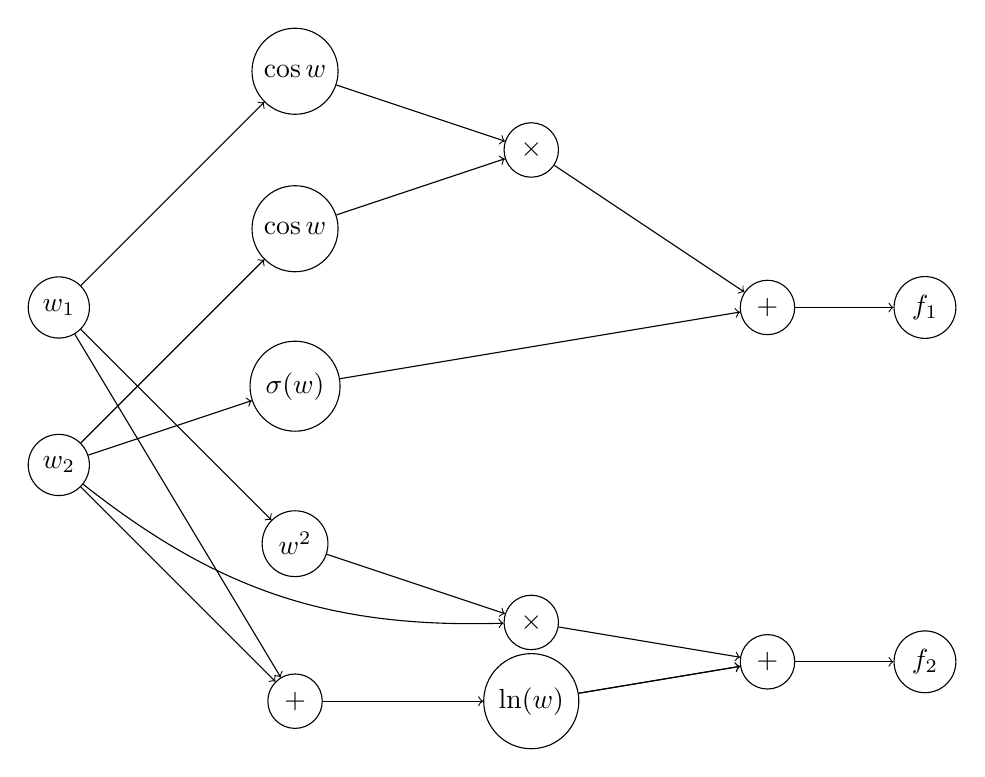
\begin{tikzpicture}
	\begin{scope}[every node/.style={circle,draw}]
		\node (w1) at (0,-2) {$w_{1}$};
		\node (w2) at (0,-4) {$w_{2}$};


		\node (cosw1) at (3, 1) {$\cos w$};
		\node (cosw2) at (3, -1) {$\cos w$};
		\node (sigmoid) at (3, -3) {$\sigma(w)$};
		\node (sq) at (3, -5) {$w^{2}$};
		\node (plusl1) at (3, -7) {$+$};

		\node (multl21) at (6, 0) {$\times$};
		\node (multl22) at (6, -6) {$\times$};
		\node (ln) at (6, -7) {$\ln(w)$};

		\node (addl31) at (9, -2) {$+$};
		\node (addl32) at (9, -6.5) {$+$};

		\node (f1) at (11, -2) {$f_{1}$};
		\node (f2) at (11, -6.5) {$f_{2}$};
	\end{scope}

	\begin{scope}
		\path[->] (w1) edge (cosw1);
		\path[->] (w1) edge (sq);
		\path[->] (w1) edge (plusl1);
		\path[->] (w2) edge (cosw2);
		\path[->] (w2) edge (sigmoid);
		\path[->] (w2) edge[bend right=20] (multl22);
		\path[->] (w2) edge (plusl1);

		\path[->] (cosw1) edge (multl21);
		\path[->] (cosw2) edge (multl21);
		\path[->] (sigmoid) edge (addl31);
		\path[->] (sq) edge (multl22);
		\path[->] (plusl1) edge (ln);

		\path[->] (multl21) edge (addl31);
		\path[->] (multl22) edge (addl32);
		\path[->] (ln) edge (addl32);
		\path[->] (ln) edge (addl32);

		\path[->] (addl31) edge (f1);
		\path[->] (addl32) edge (f2);
	\end{scope}
\end{tikzpicture}

We can then calculate the value
\begin{equation*}
	[f_{1}(1, 2), f_{2}(1, 2)] \approx [0.65595, 3.0986]
\end{equation*}

\subexercise{b}
Let $J_{i,j}$ be the entry on the $i$th row and the $j$th column of the Jacobian $J$.
We have that $J_{i,j} = \pdv{f_{i}}{w_{i}}$. Now, we find the four entries in this
matrix using numerical differentiation to be
\begin{align*}
	\pdv{f_{1}}{w_{1}} & = \frac{1}{0.01}[f_{1}(1.01, 2) - f_{1}(1, 2)] \approx 0.35129   \\
	\pdv{f_{2}}{w_{1}} & = \frac{1}{0.01}[f_{2}(1.01, 2) - f_{2}(1, 2)] \approx 4.352779  \\
	\pdv{f_{1}}{w_{2}} & = \frac{1}{0.01}[f_{1}(1, 2.01) - f_{1}(1, 2)] \approx -0.385569 \\
	\pdv{f_{2}}{w_{2}} & = \frac{1}{0.01}[f_{2}(1, 2.01) - f_{2}(1, 2)] \approx 1.332779  \\
\end{align*}

\subexercise{c}
Now, we will compute these same derivatives using forward mode auto-differentiation.
To do this, we first define $\dot{w} = \pdv{w}{t}$ where $t$ is just some parameter.
We also create intermediate variables for our computations. For $f_{1}$ we have
\begin{align*}
	u_{1} & = w_{1},         & \dot{u}_{1} & = \dot{w}_{1}                           \\
	u_{2} & = w_{2},         & \dot{u}_{2} & = \dot{w}_{2}                           \\
	u_{3} & = \cos u_{1},    & \dot{u_{3}} & = -\sin(u_{1})\dot{u_{1}}               \\
	u_{4} & = \cos u_{2},    & \dot{u_{4}} & = -\sin(u_{2})\dot{u}_{2}               \\
	u_{5} & = u_{3}*u_{4},   & \dot{u_{5}} & = \dot{u}_{3}u_{4} + u_{3}\dot{u}_{4}   \\
	u_{6} & = \sigma(u_{2}), & \dot{u_{6}} & = \sigma(u_{2})(1 - \sigma(u_{2}))u_{2} \\
	u_{7} & = u_{5} + u_{6}, & \dot{u_{7}} & = \dot{u}_{5} + \dot{u}_{6}             \\
	f_{1} & = u_{7},         & \dot{f}_{1} & = \dot{u}_{7}
\end{align*}
Repeating the same for $f_{2}$ we get
\begin{align*}
	u_{1} & = w_{1},         & \dot{u_{1}} & = \dot{w}_{1}                         \\
	u_{2} & = w_{2},         & \dot{u_{2}} & = \dot{w}_{2}                         \\
	u_{3} & = u_{1} + u_{2}, & \dot{u_{3}} & = \dot{u}_{1} + \dot{u}_{2}           \\
	u_{4} & = \ln u_{3},     & \dot{u_{4}} & = \frac{\dot{u}_{3}}{u_{3}}           \\
	u_{5} & = u_{1}^{2},     & \dot{u_{5}} & = 2u_{1}\dot{u}_{1}                   \\
	u_{6} & = u_{5}u_{2},    & \dot{u_{6}} & = \dot{u}_{5}u_{2} + u_{5}\dot{u}_{2} \\
	u_{7} & = u_{4} + u_{6}, & \dot{u_{7}} & = \dot{u}_{5} + \dot{u}_{6}           \\
	f_{2} & = u_{7},         & \dot{f_{2}} & = \dot{u}_{7}.
\end{align*}

Now, if we let $t = w_{1}$, then $\dot{w}_{1} = 1, \dot{w}_{2} = 0$, and viceversa if $t = w_{2}$.
Therefore, using both values of $t$ and propagating we get that (to 6 decimal points).
\begin{align*}
	\pdv{f_{1}}{w_{1}} & = 0.350175, \\
	\pdv{f_{2}}{w_{1}} & = 4.33333,  \\
	\pdv{f_{1}}{w_{2}} & = -0.38630, \\
	\pdv{f_{2}}{w_{2}} & = 1.33333.
\end{align*}

\subexercise{d}
Similarly to forward mode auto-differentiation, we now define $\bar{w} = \pdv{f}{w}$.
Where $f$ is some function, we again make use of the intermediate variables. For $f_{1}$
we let $f = f_{1}$ and get that.
\begin{align*}
	f_{1} & = u_{7},         & \bar{f}_{1} & = 1                                     \\
	u_{7} & = u_{5} + u_{6}, & \bar{u}_{7} & = \bar{f}_{1} =  1                      \\
	u_{6} & = \sigma(u_{2}), & \bar{u}_{6} & = \sigma(u_{2})(1 - \sigma(u_{2}))u_{2} \\
	u_{5} & = u_{3}*u_{4},   & \bar{u_{5}} & = \dot{u}_{3}u_{4} + u_{3}\dot{u}_{4}   \\
	u_{4} & = \cos u_{2},    & \bar{u_{4}} & = -\sin(u_{2})\dot{u}_{2}               \\
	u_{3} & = \cos u_{1},    & \bar{u_{3}} & = -\sin(u_{1})\dot{u_{1}}               \\
	u_{2} & = w_{2},         & \bar{u}_{2} & = \dot{w}_{2}                           \\
	u_{1} & = w_{1},         & \bar{u}_{1} & = \bar{w}_{1}                           \\
\end{align*}

Similarly, for $f = f_{2}$ we get
\begin{align*}
	f_{2} & = u_{7},         & \bar{f_{2}} & = 1,\\
	u_{7} & = u_{4} + u_{6}, & \bar{u_{7}} & = \bar{f}_{2} = 1,\\
	u_{6} & = u_{5}u_{2},    & \bar{u_{6}} & = \bar{u}_{7} = 1,\\
	u_{5} & = u_{1}^{2},     & \bar{u_{5}} & =\bar{u}_{6}u_{2} = u_{2}, \\
	u_{4} & = \ln u_{3},     & \bar{u_{4}} & =\bar{u}_{7} = 1,\\
	u_{3} & = u_{1} + u_{2}, & \bar{u_{3}} & = \bar{u}_{4} \frac{1}{u_{3}} = \frac{1}{u}_{3},\\
	u_{2} & = w_{2},         & \bar{u_{2}} & = \bar{u}_{3} * 1 = \bar{u}_{3}, \\
	u_{1} & = w_{1},         & \bar{u_{1}} & = \bar{u}_{5}*2u_{1} + \bar{u}_{3},
\end{align*}

Now, propagating, we get that (to 6 decimal points),
\begin{align*}
	\pdv{f_{1}}{w_{1}} & = 0.350175, \\
	\pdv{f_{2}}{w_{1}} & = 4.33333,  \\
	\pdv{f_{1}}{w_{2}} & = -0.38630, \\
	\pdv{f_{2}}{w_{2}} & = 1.33333.
\end{align*}

\subexercise{e}
Yes, please never put such a tedious exercise in future worksheets.

\exercise{5}
\subexercise{a}

\begin{proof}
	To show that $C_{a}S = SC_{a}$ we can simply multiply them. Multiplying the matrices we get
	\begin{equation*}
		C_{a}S =
		\begin{bmatrix}
			a_{0}     & a_{n - 1} & \cdots & a_{1}  \\
			a_{1}     & a_{0}     & \cdots & a_{2}  \\
			\vdots    & \vdots    & \ddots & \vdots \\
			a_{n - 1} & a_{n - 2} & \cdots & a_{0}
		\end{bmatrix}
		\begin{bmatrix}
			0 & 0      & \cdots & 1      \\
			1 & 0      & \cdots & 0      \\
			0 & \ddots & \ddots & \vdots \\
			0 & \cdots & 1      & 0
		\end{bmatrix}
		=
		\begin{bmatrix}
			a_{n - 1} & a_{n - 2} & \cdots & a_{0}     \\
			a_{1}     & a_{0}     & \cdots & a_{1}     \\
			\vdots    & \vdots    & \ddots & \vdots    \\
			a_{n - 2} & a_{n - 3} & \cdots & a_{n - 1}
		\end{bmatrix}
		= SC_{a}
	\end{equation*}
\end{proof}

\subexercise{b}
\begin{proof}
	Let $f$ be a linear operation. We want to show that $f(S\bm{x}) = Sf(\bm{x}) \iff f(x) = (x * w)_{i} = C_{a}\bm{x}$.

	($\Leftarrow$)
	We assume that $f(\bm{x}) = C_{a} \bm{x}$, as we proved in (a) we know that $C_{a}S = SC_{a}$.
	Therefore, we have that
	\begin{equation*}
		f(S \bm{x}) = C_{a}S \bm{x} = SC_{a}\bm{x} = Sf(\bm{x}).
	\end{equation*}
	Thus, $f$ is shift-equivariant.

	($\Rightarrow$)
	We assume that $f$ is some shift-equivariant linear operation.
	This implies that $f(S \bm{x}) = AS \bm{x} = SA \bm{x} = Sf(x)$.

	Let $A$ be any matrix (linear operation), then we have that
	\begin{equation*}
		AS =
		\begin{bmatrix}
			a_{11} & a_{12} & \cdots        & a_{1n} \\
			a_{21} & a_{22} & \cdots        & a_{2n} \\
			\vdots & \vdots & \ddots        & \vdots \\
			a_{n1} & a_{n2} & \cdots a_{nn}
		\end{bmatrix}
		\begin{bmatrix}
			0 & 0      & \cdots & 1      \\
			1 & 0      & \cdots & 0      \\
			0 & \ddots & \ddots & \vdots \\
			0 & \cdots & 1      & 0
		\end{bmatrix}
		=
		\begin{bmatrix}
			a_{12} & a_{13} & \cdots & a_{1n}       & a_{11} \\
			a_{22} & a_{23} & \cdots & a_{n, n - 1} & a_{21} \\
			\vdots & \vdots & \ddots & \vdots       & \vdots \\
			a_{n2} & a_{3n} & \cdots & a_{nn}       & a_{n1}
		\end{bmatrix}
	\end{equation*}
	Now, by our assumption, we know this must be equal to
	\begin{align*}
		SA
		 & =
		\begin{bmatrix}
			0 & 0      & \cdots & 1      \\
			1 & 0      & \cdots & 0      \\
			0 & \ddots & \ddots & \vdots \\
			0 & \cdots & 1      & 0
		\end{bmatrix}
		\begin{bmatrix}
			a_{11} & a_{12} & \cdots        & a_{1n} \\
			a_{21} & a_{22} & \cdots        & a_{2n} \\
			\vdots & \vdots & \ddots        & \vdots \\
			a_{n1} & a_{n2} & \cdots a_{nn}
		\end{bmatrix}, \\
		 & =
		\begin{bmatrix}
			a_{n1}       & a_{n2}       & \cdots & a_{n, n-1}     & a_{nn}       \\
			a_{11}       & a_{12}       & \cdots & a_{1, n - 1}   & a_{1n}       \\
			\vdots       & \vdots       & \ddots & \vdots         & \vdots       \\
			a_{n - 1, 1} & a_{n - 1, 2} & \cdots & a_{n - 1, n-1} & a_{n - 1, n}
		\end{bmatrix}.
	\end{align*}
	We can see now that this implies that $a_{11} = a_{22} = \dots = a_{nn}$,
	$a_{12} = a_{n1} = \dots$. We now see that this is nothing
	but the circulant matrix.

	Therefore, we have that the circulant matrix is the only linear operator that
	is shift-equivariant.
\end{proof}

\subexercise{c}
Shift-equivariance is very powerful in terms of processing spatial or spatio-temporal data.
This is because it implies that the data can be shifted in any direction, and the result
will be the same as if it were shifted \textit{after} the convolution.

This means, in short, that the convolution kernel is not dependent on spatial location,
which makes it generalise easily.

\exercise{6}
No, SGD is not guaranteed to decrease every iteration.

Let $\bm{w}^{t} = 0$. We have that,
\begin{equation*}
    f(\bm{w}^{t}) = \frac{1}{2}[(-2)^{2} + 1^{2}] = \frac{5}{2}.
\end{equation*}

Now, we calculate $\bm{w}^{t + 1}$ and pick the term $\frac{1}{2}(\bm{w} + 1)^{2}$.
Therefore, we have that
\begin{equation*}
    \bm{w}^{t+1} = \bm{w}^{t} - \eta \grad \frac{1}{2}(\bm{w} + 1)^{2} |_{\bm{w} = \bm{w}^{t}}
    = 0 - \eta(w^{t} + 1) = -\eta.
\end{equation*}

Plugging this back into the objective function we get 
\begin{equation*}
    f(\bm{w}^{t+1}) = \frac{1}{2}[(-\eta - 2)^{2} + (-\eta + 1)^{2}]
    = \eta^{2} + \eta + \frac{5}{2} \geq \frac{5}{2},
\end{equation*}
since $\eta > 0$. We can see that we have increased the overall loss.


\exercise{7}
\subexercise{a}
The key contribution of this paper is the fact that neural networks are able to fit anything,
even random noise. The idea is that a neural network with enough layers can represent any function,
therefore the representational power of deep neural networks is huge. Thus, they are able to attain
very low test accuracies on datasets with the labels completely randomised. This puts into question
how one is to understand the generalisation power of neural networks. It begs the question,
if the network can learn random noise, is it really learning anything? This more of a philosphical
question than anything else, but it does give rise to even more mystery into how deep neural networks
work.

\subexercise{b}
My biggest takeaway from this paper is that, given a neural network with enough parameters (more than 
datapoints), it is able to completely memorise what the output is. Therefore, it is important to take 
this into account when thinking about the generalisation of the model. I think it is clear that more work
needs to be done in how we measure the representational power of models. This is because once we can 
generalise the representation of a model we can understand what it is able to brute-force memorise.

\end{document}
